\section{Inleiding}

Communicatie met een ruimtetuig (voor bijvoorbeeld een Marsmissie) is cruciaal voor de goede werking van een verblijf in de ruimte om verschillende redenen. Enerzijds superviseert het controlecentrum op aarde de werking van de missie aan de hand van de resultaten van proeven, foto’s, meetwaarden, ... en anderzijds geeft het opdrachten door aan de bemanning en bestuurt het ruimtetuig.

De enige manier om te communiceren met een toestel in de ruimte zijn radiogolven.

Dit rapport gaat over een aantal principes om deze communicatie te realiseren. In een eerste deel gaat het over een beschrijving van het ‘Deep Space Network’ met het doel en de werking van de up- en downlink. In een tweede deel gaat het dieper in op fundamentelere onderwerpen zoals allereerst “Wat zijn radiogolven en hoe bevatten deze de informatie?”, vervolgens op “Hoe werken schotelantennes?” om te eindigen met “Waarom is communicatie met ruimtetuigen op grote afstand moeilijk?”.

\section{Communicatie met een ruimtemissie}

\subsection{Wat is het 'Deep Space Network'?}

Het ‘Deep Space Network’ (DSN), dat sinds 1958 als een onderdeel van NASA (National Aeronautics and Space Administration) bestaat, is een internationaal netwerk dat door middel van drie gigantische antennes op de aarde communicatie mogelijk maakt met satellieten of ruimtetuigen \cite{martin}. Het eerste deep-space communicatiecentrum is te vinden in de Mojave-woestijn in Californië nabij Goldstone, een tweede nabij Madrid in Spanje en een derde in Canberra, Australië. Door deze geografische spreiding, telkens ongeveer 120° verder op de aardbol, is steeds communicatie mogelijk met om het even waar in de ruimte \cite{christiaens}. 

\subsection{Wat is de uplink en de downlink bij een 'Deep Space Network'?}

De uplink is het verzenden van informatie vanop aarde naar een ruimtetuig. De uplink doet een upload. De downlink gaat in de andere richting: van een ruimtetuig naar de aarde. Deze doet een download. De vertraging is de tijd die verstrijkt tussen het verzenden en ontvangen van een signaal. Radiogolven zijn, net zoals licht, elektromagnetische golven. De voortplantingssnelheid is voor radiogolven 3.108 meter per seconde in lucht of het luchtledige. Dit lijkt snel, maar is eigenlijk (relatief) traag wegens de enorme te overbruggen afstanden \cite{updown}. Deze afstand is bijvoorbeeld gemiddeld 384 450 km tot de maan \cite{maan} en 230 000 000 km tot Mars \cite{mars}.

\subsection{Wat zijn radiogolven en hoe bevatten deze informatie?}

Elektromagnetische golven zijn, op basis van hun frequentie of golflengte, onder te verdelen in radiogolven, microgolven, lichtstralen, röntgenstralen, gammastraling, … \cite{radiowaves}, zoals te zien in figuur \ref{fig:EMS} op bladzijde \pageref{fig:EMS}.

\begin{figure}[ht]
  \centering
  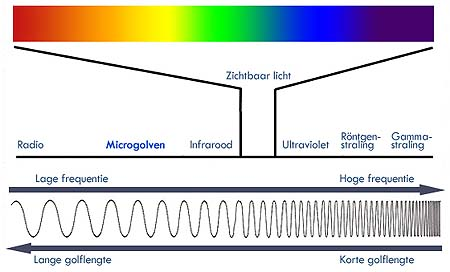
\includegraphics[width=0.5\textwidth]{voorbeeld_figuren/spectrum_straling}
  \caption{Elektromagnetische straling.} 
  \cite{energiezonnepanelen} %Als je deze cite in de caption plaatst, komt de referentie ook in de lijst van figuren voor en is de volgorde niet juist.
  \label{fig:EMS}
\end{figure}

De frequentie f van radiogolven is het aantal keer per seconde dat het signaal maximaal wordt. De eenheid van frequentie is Hz (Hertz). De golflengte is de afstand tussen één maximum en het volgende maximum van het signaal. De elektrische en magnetische component en voortplantingsrichting zijn te zien in figuur \ref{fig:golf} op bladzijde \pageref{fig:golf}.

\begin{figure}[ht]
  \centering
  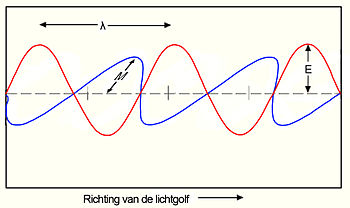
\includegraphics[width=0.5\textwidth]{voorbeeld_figuren/elektromagnetische_golf}
  \caption{Voortplanting elektromagnetische golf.} 
  \cite{elektromagnetischestraling}
  \label{fig:golf}
\end{figure}

Een zeer belangrijk verband tussen de frequentie f en de golflengte $\lambda$ is: $v = f\lambda$, met v de voortplantingssnelheid van de golf \cite{elektromagnetischestraling}. Bij een grotere golflengte zijn de golven immers breder en duurt het dus langer eer een volledige golf ergens voorbij komt (lagere frequentie). Deze tijd is de periode T. Er geldt: $T = \frac{1}{f}$. De golflengte van zichtbaar licht is (veel) kleiner dan van radiogolven: ordegrootte $10^{-6}$ meter. 

Radiogolven voor radio en TV hebben dan weer een grotere golflengte dan radiogolven voor communicatie in de ruimte. Bij deze laatste  is de golflengte zeer klein: ongeveer één centimeter. 

\begin{figure}[ht]
  \centering
  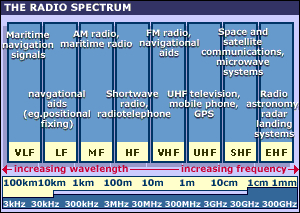
\includegraphics[width=0.5\textwidth]{voorbeeld_figuren/radiospectrum}
  \caption{Radiospectrum.} 
  \cite{wavelengths}
  \label{fig:radiospectrum}
\end{figure}

Een radiogolf voldoet aan de uitdrukking: 
\begin{equation*} %eventueel \label{} bijvoegen om te kunnen refereren.
v = A\sin(\omega t+\phi)
\end{equation*}	%equation zonder * geeft een nummer bij de uitdrukking. Dit is nodig als je naar deze formule wil refereren. 
Dit impliceert dat een golf informatie kan bevatten door ofwel de amplitude A ofwel de hoek $(\omega t+\phi)$ ofwel eventueel een combinatie van amplitude en hoek te veranderen. Bij amplitudemodulatie (AM) bevat de amplitude de informatie en bij frequentiemodulatie (FM) is dat $\omega$ \cite{radiowaves1}.  Hierbij is $\omega = 2\pi f$. Een variante op frequentiemodulatie is fasemodulatie (PM). Bij fasemodulatie is de fase een functie van het door te sturen signaal.

\subsubsection{Amplitudemodulatie}

Bij amplitudemodulatie \cite{kennedy} (AM) is de golfvorm het resultaat van een hoogfrequent signaal, de draaggolf met een vaste frequentie, waarvan de amplitude veranderlijk is naargelang de door te zenden informatie. Een positief (audio)signaal levert een iets hogere draaggolfamplitude, een negatief signaal levert een iets lagere draaggolfamplitude. Wiskundig is de amplitude van de draaggolf gelijk aan de som van een constant signaal (gelijkspanning) met het door te zenden signaal. De mate waarin de draaggolf het bronsignaal volgt, heet de modulatiediepte, uitgedrukt in procenten van de ongemoduleerde draaggolf. Deze is steeds kleiner dan 1. Figuur \ref{fig:AM} op bladzijde \pageref{fig:AM} toont een informatiesignaal, de ongemoduleerde draaggolf (carrier in het Engels) en ten slotte het resulterend signaal.

\begin{figure}[ht]
  \centering
  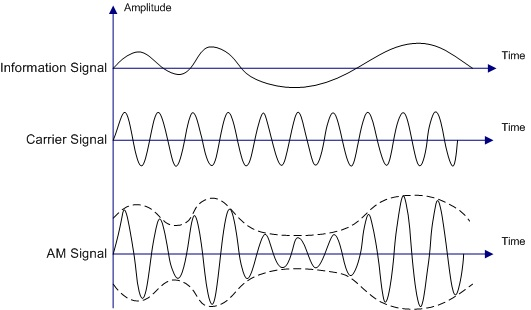
\includegraphics[width=0.5\textwidth]{voorbeeld_figuren/AM}
  \caption{AM modulatie.} 
  \cite{AM}
  \label{fig:AM}
\end{figure}

\subsubsection{Frequentiemodulatie} 

Bij frequentiemodulatie \cite{kennedy} (FM) is de bekomen golfvorm opnieuw het resultaat van een hoogfrequent signaal, de draaggolf, maar waarbij nu de amplitude constant is en de frequentie veranderlijk naargelang de door te zenden informatie. Hoe hoger de amplitude van het door te zenden signaal, hoe hoger de frequentie van de aangepaste draaggolf. Frequentiemodulatie is minder gevoelig aan ruis dan amplitudemodulatie. Daar staat wel tegenover dat een FM-signaal bij een gegeven bronsignaal in het algemeen, afhankelijk van de modulatie-index, veel meer bandbreedte nodig heeft dan een AM-signaal. Figuur \ref{fig:FM} op bladzijde \pageref{fig:FM} toont een informatiesignaal, de ongemoduleerde draaggolf (carrier in het Engels) en ten slotte het resulterend signaal (de gemoduleerde draaggolf).

\begin{figure}[ht]
  \centering
  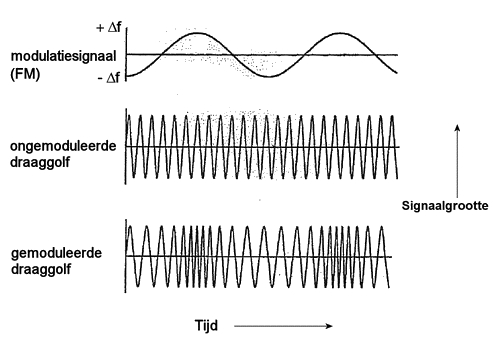
\includegraphics[width=0.5\textwidth]{voorbeeld_figuren/FMwit}
  \caption{FM modulatie.} 
  \cite{FM}
  \label{fig:FM}
\end{figure}


\subsection{Hoe werken schotelantennes?}

Elk type antenne heeft zijn toepassingsgebied. Voor communicatie met een ruimtetuig, zijn alleen schotelantennes bruikbaar \cite{kennedy}. De reden hiervoor is dat alleen schotelantennes hun energie in één welbepaalde enge bundel kunnen verzenden.

\begin{figure}[ht]
  \centering
  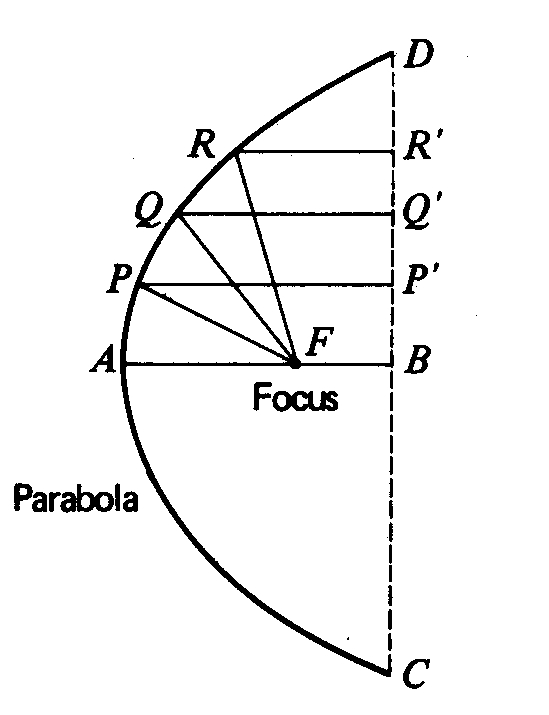
\includegraphics[width=0.3\textwidth]{voorbeeld_figuren/paraboolantenne_doorsnede}
  \caption{Doorsnede van een paraboolantenne.} 
  \cite{kennedy}
  \label{fig:parabool}
\end{figure}

Schotelantennes hebben een parabolische vorm, zoals te zien in figuur \ref{fig:parabool} op bladzijde \pageref{fig:parabool}. Een eigenschap van deze vorm is dat alle signaalenergie die erop invalt, wordt geconcentreerd in het brandpunt (focus) en omgekeerd dat alle energie die vertrekt vanuit het brandpunt naar de parabool, verder reist in een zeer gericht signaal. 

Kenmerkend voor schotelantennes is dat ze werken bij hoge frequenties en bijgevolg kleine golflengten.

Een antenne heeft als doel zoveel mogelijk het signaal in één richting te sturen. Dit lukt beter naarmate de golflengte kleiner en de antenne groter is. Communicatie in de ruimte vereist bijgevolg kleine golflengten en dus hoge frequenties. De antennes voor het Deep Space Network zijn bovendien zeer groot!

\subsection{Waarom is communicatie met ruimtetuigen op grote afstand moeilijker?}

De oppervlakte van een bol is gelijk aan $4\pi r^{2}$. Het ontvangen signaal op een bepaalde afstand r van de antenne is bijgevolg omgekeerd evenredig met $r^{2}$ of dus evenredig met $r^{-2}$. Wanneer de afstand dus verdubbelt, verkleint het vermogen van het signaal al vier keer! 

In het geval van communicatie met een ruimtetuig is de afstand zeer groot. Het ontvangen signaal is bijgevolg zeer klein en dus moet de schotelantenne zeer groot zijn om toch maar voldoende invallend vermogen te kunnen verzamelen in het brandpunt \cite{radiocontact}. Een voorbeeld hiervan is figuur \ref{fig:effelsberg} op bladzijde \pageref{fig:effelsberg}.

\begin{figure}[ht]
  \centering
  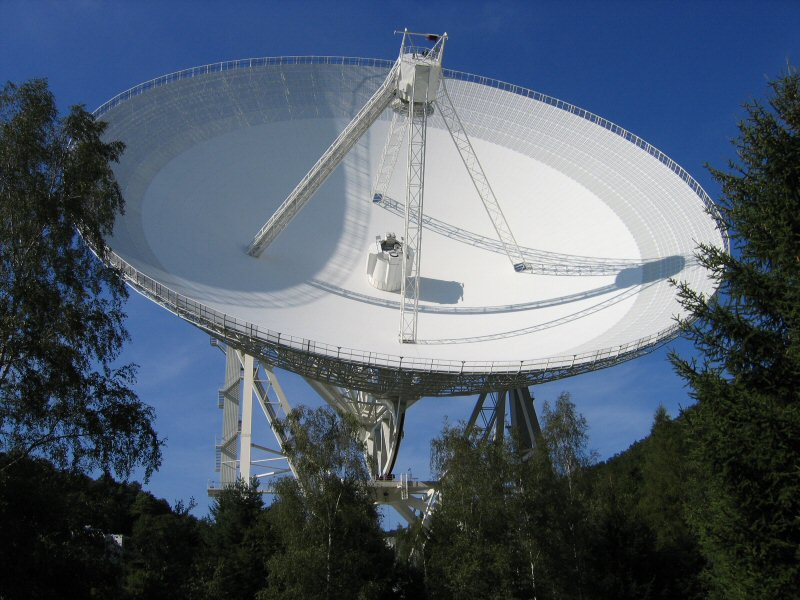
\includegraphics[width=0.6\textwidth]{voorbeeld_figuren/paraboolantenne}
  \caption{Effelsberg telescoop.} 
  \cite{effelsberg}
  \label{fig:effelsberg}
\end{figure}

\section{Geplande ruimtevluchten}

Een overzicht van toekomstige ruimtemissies naar de maan kan je vinden in tabel \ref{tab:missies} op bladzijde \pageref{tab:missies}.

\begin{table}[ht]
\centering
\small
\begin{tabular}{cc|c} %De | duidt aan waar je een verticale lijn in de tabel wil.
Land &Jaar &Missie \\ \hline
India &2018 &Chandrayaan-2 \\ 
Verenigde Staten &2018 &Lunar Flashlight \\ 
Verenigde Staten &2018 &Lunar Ice Cube \\ 
Japan &2019 &SLIM \\
Zuid-Korea &2020 &Moon orbiter \\ 
Verenigd Koninkrijk &2024 &Lunar Mission One \\
\end{tabular}
\caption{Land, jaartal en naam van enkele toekomstige missies.}
\cite{missies}
\label{tab:missies}
\end{table}

\section{Besluit}

Communicatie met een missie naar Mars is zeker mogelijk dankzij de zeer grote schotelantennes van het ‘Deep Space Network’. Deze antennes kunnen permanent voldoende sterke signalen uit de ruimte ontvangen of naar de ruimte versturen dankzij hun grote afmetingen, hun geografische spreiding en de gebruikte frequenties. Amplitudemodulatie of frequentiemodulatie zijn bruikbare technieken om de signalen uit te zenden of te ontvangen.